\subsection{Bondi et al.}
About 10 years after the PRNU-based method for digital camera identification, in 2017, the authors of ``First Steps Toward Camera Model Identification with Convolutional Neural Networks" investigated a novel approach to solve the camera model identification problem, based on Convolutional Neural Networks. The choice was fully motivated by other successful deep-learning algorithms applied to forensics tasks.
In particular, they made use of a \textit{Convolutional Neural Network} (CNN) which learns the features characterizing each camera model directly from the acquired images, rather than using handcrafted features. In addition, they also used linear \textit{Support Vector Machines} (SVMs) for classification.

\begin{figure}[ht]
	\centering
	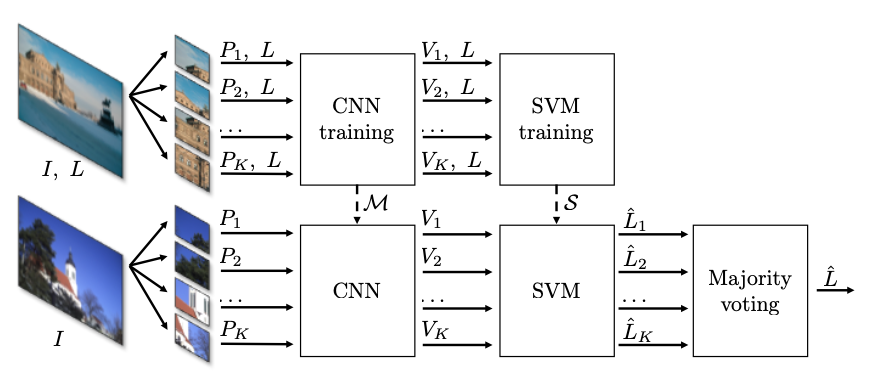
\includegraphics[keepaspectratio, width=0.5\textwidth]{CNNSVM}
	\caption{CNN - SVM architecture | training and evaluation pipelines}
	\label{fig:CNNSVM}
\end{figure}

As shown in Fig. \ref{fig:CNNSVM}, given a set of training and validation labeled samples coming from \textit{N} known camera models, the training proceeds as follows:
for each image \textit{I} with the corresponding label \textit{L} (camera model), \textit{K} non overlapping patches are extracted, where each patch \textit{P\textsubscript{k}} inherits the same label \textit{L} of the source image. For each patch, the CNN extracts a feature vector \textit{V\textsubscript{k}} of 128 elements. The resulting feature vectors are then used to train a battery of $ N \cdot (N - 1)/2 $ linear binary SVM classifiers \textit{S}. 
During evaluation, the battery \textit{S} of linear SVMs assigns a label $\hat{L}$\textit{\textsubscript{k}} to each patch. The predicted label $\hat{L}$ for image \textit{I} is obtained through majority voting on $\hat{L}$\textit{\textsubscript{k}}, $k \in [1, K]$.

The advantages of the proposed CNN are mainly two:
\begin{itemize}
	\item It learns a feature extraction methodology that generalizes well on a set of unknown camera models;
	\item The resulting feature vectors have only 128 elements, allowing to characterize camera models in a space with reduced dimensionality and  consequently enabling the use of simple classifiers like SVMs.
\end{itemize}

